\documentclass{article}
  % Packages and package settings
  \usepackage{fontspec}
    \setmainfont{Charis SIL}
  \usepackage{hyperref}
    \hypersetup{colorlinks=true,
                allcolors=blue}
  \usepackage{caption}
  \usepackage{graphicx}
    \graphicspath{{./figures/}}

  % Title info
  \author{Joshua McNeill}
  \title{Homework 4}
  \date{\today}

  % Custom commands
  \newcommand{\lexi}[1]{\textit{#1}}
  \newcommand{\regfig}[2]{
    \begin{minipage}[t]{\linewidth}
      \captionof{figure}{#1}
      \label{fig:#2}
      \centering
      \includegraphics[scale=0.65]{#2.jpg}
    \end{minipage}
  }

\begin{document}
  \maketitle
  \begin{enumerate}
    \item
    \begin{minipage}[t]{\linewidth}
      \captionof{figure}{Significant date in American History with notes}
      \label{fig:spectronotes}
      \centering
      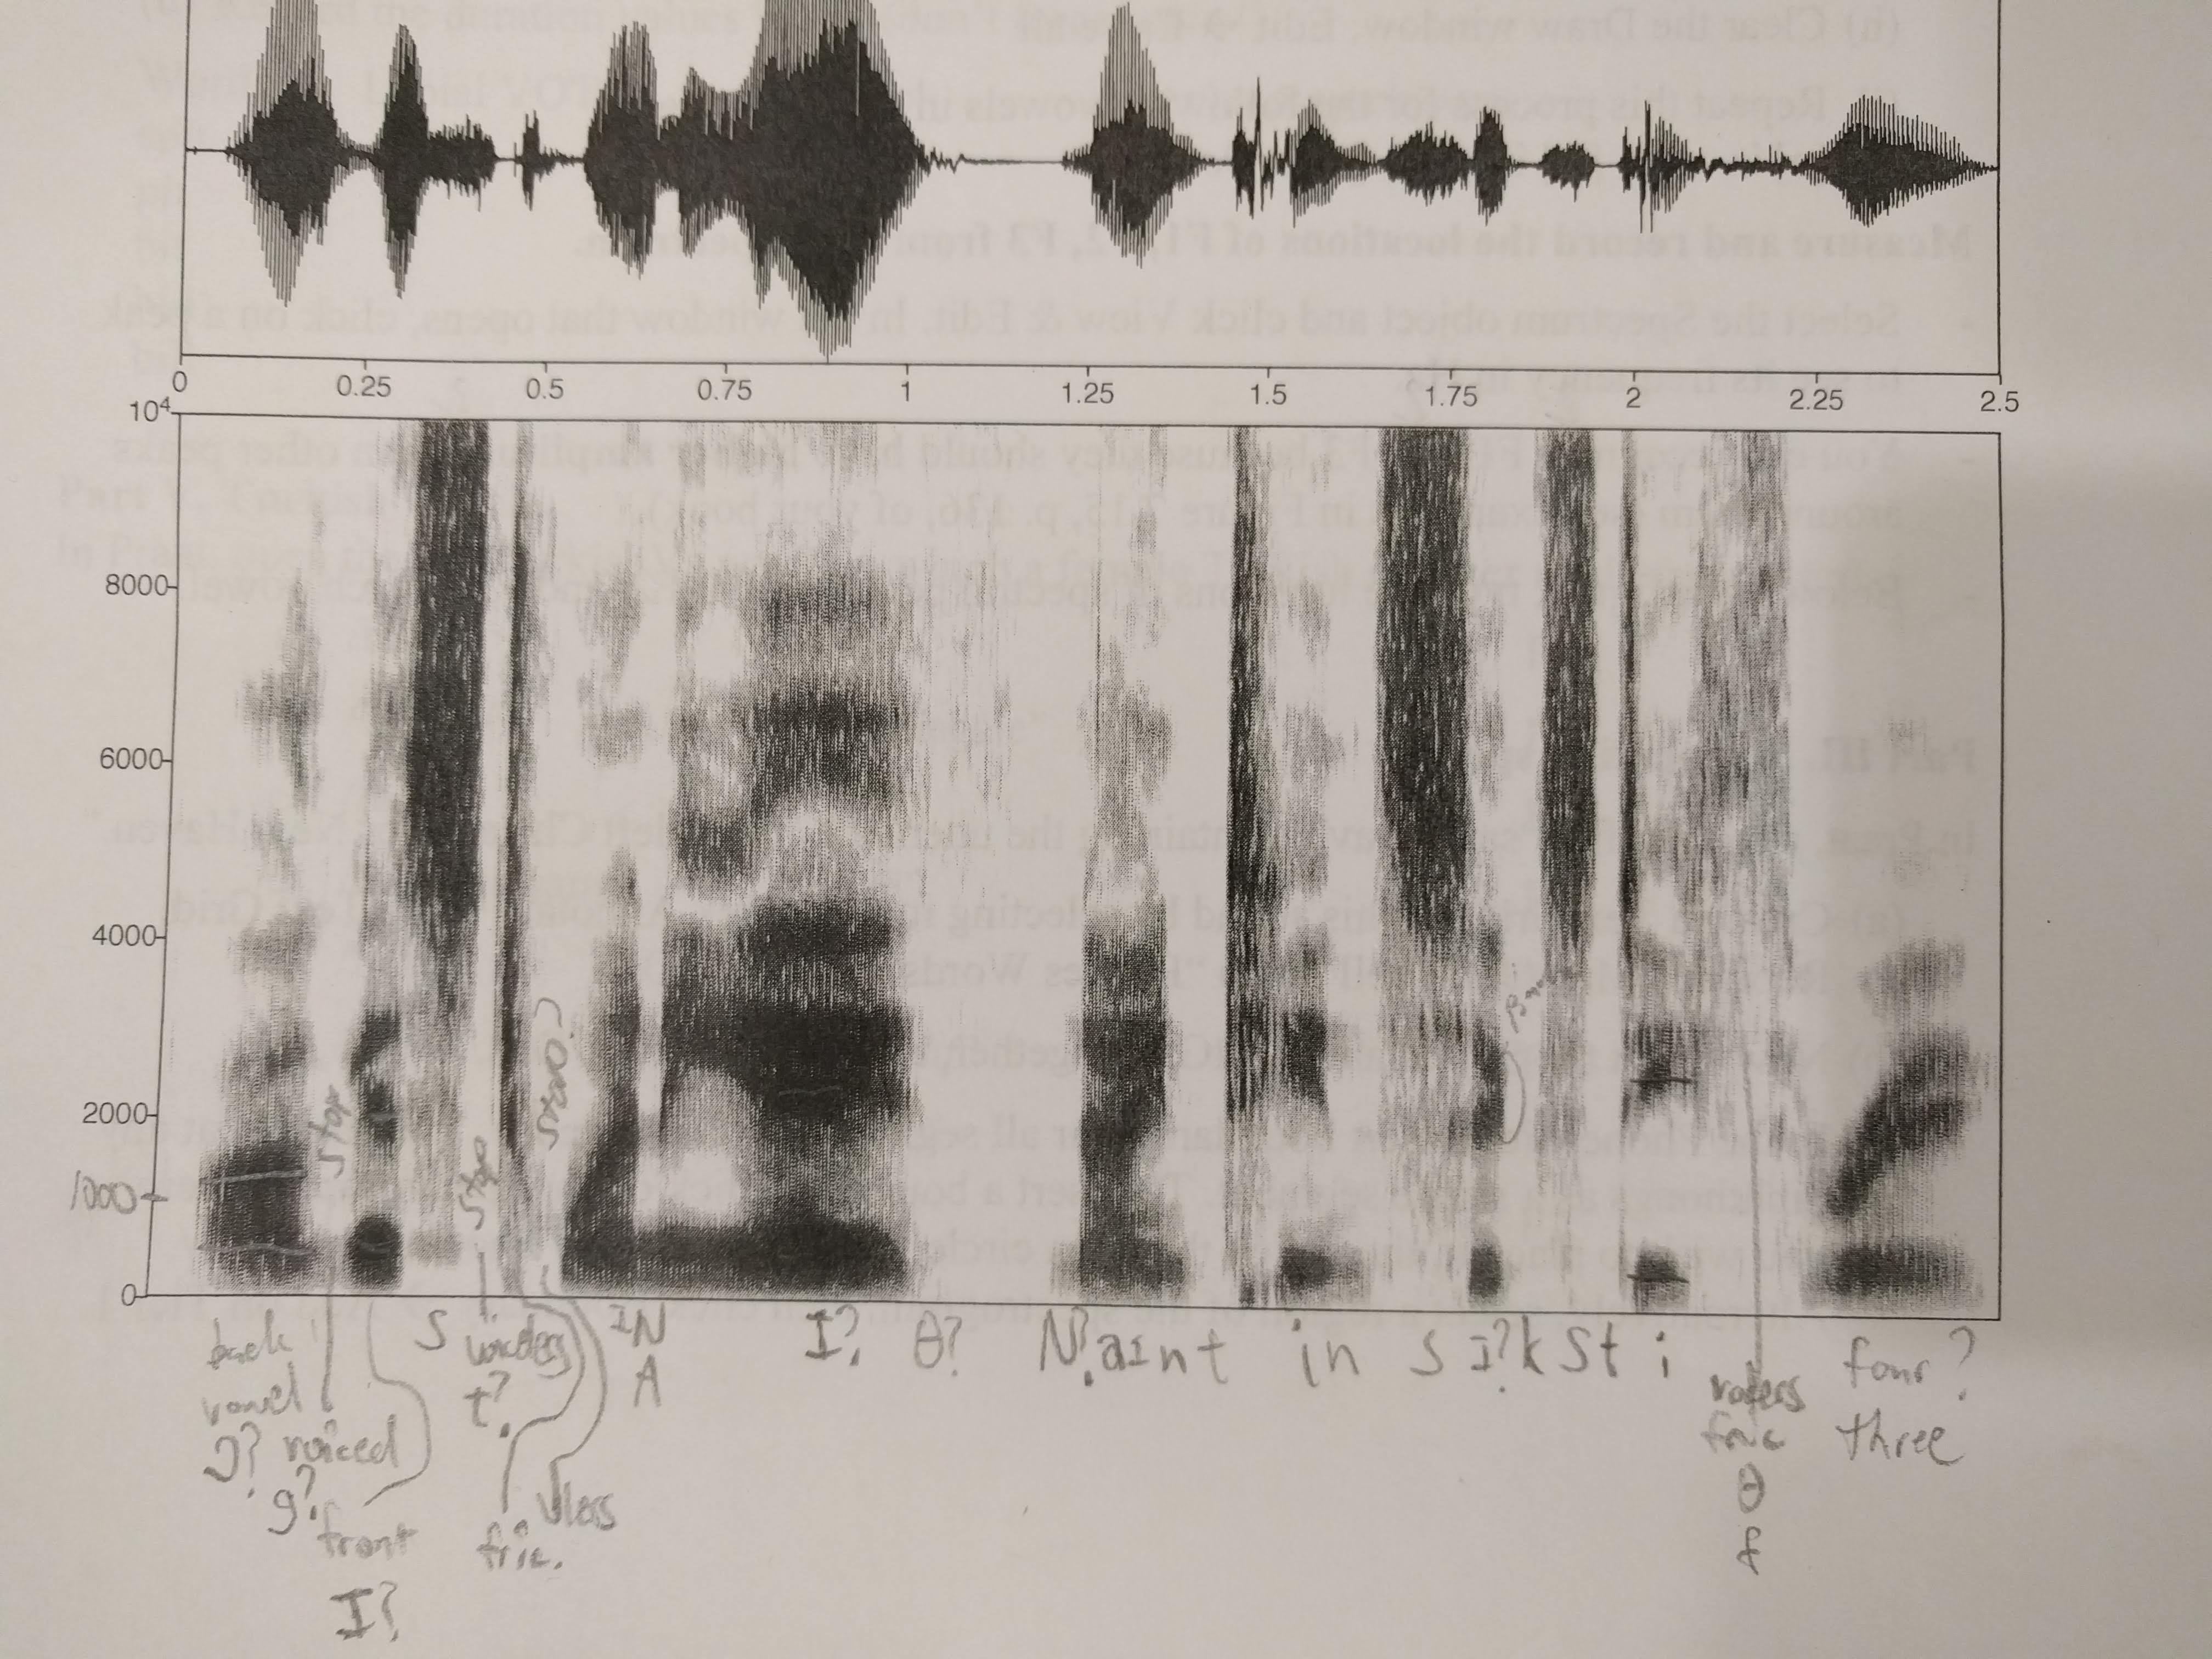
\includegraphics[scale=0.075]{spectronotes.jpg}
    \end{minipage}
    The date being pronounced in Figure \ref{fig:spectronotes} is `August 28th, 1963' or the day Martin Luther King, Jr. gave his `I Have a Dream' speech.

    \item
    \regfig{[i] in \lexi{he}}{ispectrum}
    The spectral peaks of the first three formants of [i] in Figure \ref{fig:ispectrum} are 338Hz (F1), 2993Hz (F2), and 3587Hz (F3).

    \regfig{[e] in \lexi{may}}{espectrum}
    The spectral peaks of the first three formants of [e] in Figure \ref{fig:espectrum} are 622Hz (F1), 2512Hz (F2), and 3194Hz (F3).

    \regfig{[æ] in \lexi{map}}{aespectrum}
    The spectral peaks of the first three formants of [æ] in Figure \ref{fig:aespectrum} are 1020Hz (F1), 2002Hz (F2), and 3194Hz (F3).

    \regfig{[ɔ] in \lexi{Bobby}}{ospectrum}
    The spectral peaks of the first three formants of [ɔ] in Figure \ref{fig:ospectrum} are 590Hz (F1), 1161Hz (F2), and 2863Hz (F3).
    \item
    \regfig{Sapir segmentation}{sapir}
    \item
    \begin{minipage}[t]{\linewidth}
      \captionof{table}{Durations of VOTs, vowels, and closures}
      \label{tab:vot}
      \centering
      \begin{tabular}{l | r r r}
        Word        & VOT (ms)  & Vowel (ms)  & Closure (ms) \\
        \hline
        \lexi{spit} & 20        & 129         & 90 \\
        \lexi{pit}  & 85        & 129         & 88 \\
        \lexi{bit}  & 19        & 150         & 86 \\
        \lexi{bid}  & 19        & 194         & 50 \\
        \lexi{bill} & 15        & 110         & N/A
      \end{tabular}
    \end{minipage}
    \item
    \begin{minipage}[t]{\linewidth}
      \captionof{table}{Turkish vowel formants}
      \label{tab:turkVs}
      \centering
      \begin{tabular}{l l | r r}
        Word          & Gloss       & F1 (Hz) & F2 (Hz) \\
        \hline
        /bil/         & know        & 564     & 2359 \\
        /bylbyl/      & nightingale & 514     & 2016 \\
        /bul/         & find        & 413     & 887 \\
        /bɯldɯrdʒɯn/  & quail       & 473     & 1310 \\
        /bel/         & waist       & 745     & 1835 \\
        /bol/         & plentiful   & 594     & 957 \\
        /bøl/         & divide      & 584     & 1502 \\
        /bal/         & honey       & 715     & 1209
      \end{tabular}
    \end{minipage}
    \regfig{Turkish vowels}{turkVs}
  \end{enumerate}
\end{document}
